\documentclass[11pt]{article}

\usepackage[utf8]{inputenc}
\usepackage[T1]{fontenc}
\usepackage[margin=1in]{geometry}
\usepackage{amsmath,amssymb}
\usepackage{booktabs}
\usepackage{hyperref}
\usepackage{float}
\usepackage{algorithm}
\usepackage{algpseudocode}
\usepackage{graphicx}
\usepackage{xcolor}
\usepackage{microtype}
\usepackage{parskip}

\hypersetup{
  colorlinks=true,
  linkcolor=blue!70!black,
  citecolor=blue!70!black,
  urlcolor=blue!70!black,
}

\title{\textbf{PoR-Chain: Cryptographically Anchored Cumulative Hash Chains\\
for Provable Multimedia Authenticity}}

\author{
  Sungho Kim\\
  KANT Labs\\
  \texttt{sh@kantlabs.com}
}

\date{May 18, 2026}

\begin{document}

\maketitle

\begin{abstract}
The proliferation of generative AI has eroded public trust in multimedia content,
with deepfakes increasingly used in financial fraud, political disinformation, and
fabricated evidence. Existing provenance frameworks such as the Coalition for
Content Provenance and Authenticity (C2PA)~\cite{c2pa} rely on metadata signing
schemes that fail to verify capture authenticity once a trusted device is
compromised, while sensor fingerprinting techniques such as Photo Response
Non-Uniformity (PRNU)~\cite{prnu} are vulnerable to trained adversaries. We present \textbf{PoR-Chain}, a cryptographic
framework that binds multimedia content to a specific moment in time and a specific
physical capture device through a physical feedback path that no software-only
adversary can reproduce. The foundation---\emph{Proof-of-Reality (PoR)}---embeds
time-varying data sourced from a distributed ledger into multimedia content via an
optical, acoustic, or electrical signal path during capture; the resulting content
cannot be synthesized in advance because the embedded signal would not match the
ledger state at any point prior to capture. PoR-Chain anchors a single initial blockhash and generates a SHA-256 chain that is
encoded sequentially into successive content groups, providing both single-query
verification and tamper-evident sequence integrity for continuous video. Bidirectional
time bounding, achieved by recording a termination anchor on the ledger, constrains
the time window in which content could have been generated and breaks the economic
feasibility of post-hoc synthesis attacks. We describe a working implementation
using Solana and a transparent OLED panel, and
analyze adversarial scenarios including deepfake injection, frame splicing, lipsync
forgery, and AI voice cloning. The PoR framework is described in full in a companion
paper~\cite{por}; this paper focuses on PoR-Chain and its integration with
PoR for continuous video.
\end{abstract}

\smallskip
\noindent\textbf{Keywords:} proof-of-reality, content provenance, deepfake detection, physical
unclonable functions, blockchain anchoring, hash chains, multimedia authentication


% ===========================================================================
\section{Introduction}
% ===========================================================================

Generative AI has eroded trust in multimedia content faster than forensic detection
can keep pace. The companion paper~\cite{por} surveys existing provenance approaches---
device-signing schemes, sensor fingerprinting, watermarking, and blockchain
timestamping---and shows that none verifies the \emph{act of capture} itself.
That paper introduces the Proof-of-Reality (PoR) framework, which closes this gap
for still images by binding content to a live ledger signal through a physical
feedback path.

\textbf{Hash chains.} Cryptographic hash chains as one-way commitment structures
date to Lamport~\cite{lamport}. PoR-Chain uses them as a sequence integrity
primitive bound to a ledger state, providing tamper-evident ordering across content
groups with a single ledger query---distinguishing this application from traditional
uses in authentication tokens.

This paper extends PoR to continuous video through \textbf{PoR-Chain}. The
extension rests on two complementary insights:

\begin{enumerate}
\item \textbf{Physical feedback paths cannot be simulated retroactively.} If content
  must embed a signal broadcast through a physical channel and re-captured by the
  same device, no purely software adversary can synthesize valid content---because
  the signal depends on data that was not knowable before capture.

\item \textbf{Hash chains anchored to a single ledger state provide efficient
  sequence integrity.} A single anchor blockhash seeds a SHA-256 chain encoded into
  successive content groups. Verification requires a single ledger query and local
  recomputation; any deletion, reordering, or substitution of content groups breaks
  the chain.
\end{enumerate}

% ===========================================================================
\section{PoR-Chain Framework}
\label{sec:framework}

\subsection{PoR Framework}
\label{sec:por}
% ===========================================================================

The PoR framework is described in full in the companion paper~\cite{por}. In brief:
during capture, time-varying data $D(t)$---specifically, the Solana blockhash for
the active slot, unpredictable before time~$t$---is broadcast through a physical
signal path (optical, acoustic, or electrical) and re-captured by the same device
recording the content. The captured content thus embeds $D(t)$ at the moment of
capture. Verification confirms that the embedded signal matches the ledger and that
the on-chain receipt was submitted within a configurable freshness window~$W$ of the
embedded slot. $W$ is the key security parameter: pre-synthesis is defeated by the
unpredictability of $D(t)$, and real-time synthesis is defeated as long as the
adversary cannot synthesize and submit a valid receipt within~$W$.

Two limitations of the base framework motivate PoR-Chain:
\begin{enumerate}
  \item \textbf{Transaction cost.} Each content group must be individually anchored
    on the blockchain, requiring as many on-chain transactions as there are captured
    groups. This scales linearly with content duration and is prohibitively expensive
    for long recordings.
  \item \textbf{Sequence integrity.} Detecting deletion or reordering of content
    groups requires comparing decoded signals against an independently retrieved
    sequence of $D(t)$ values, which is brittle under network jitter or partial
    decoding failures.
\end{enumerate}

% ===========================================================================
\subsection{PoR-Chain Extension}
\label{sec:rhc}
% ===========================================================================

PoR-Chain addresses both transaction cost and sequence integrity by deriving a
cryptographic chain from the blockhash $H_0$ already fetched by PoR's ledger
challenge.

\subsubsection{Chain Generation}

Using $H_0$ as the seed, the device maintains a single running SHA-256 hasher
updated with each successive content group:
\begin{equation}
  H_n = \operatorname{SHA256}(H_0 \,\|\, F_1 \,\|\, F_2 \,\|\, \cdots \,\|\, F_n)
  \label{eq:chain}
\end{equation}%
where $F_n$ denotes the $n$-th content group. For multimedia content, $F_n = V_n \| A_n$
is the concatenation of the synchronized video frame group $V_n$ and audio chunk $A_n$;
for single-channel content, $F_n$ is the frame group or audio chunk alone.
The hash is computed incrementally without re-hashing prior state, so each $H_n$
requires only one additional block operation. Any modification to $F_k$ for
$k \leq n$ changes $H_n$ and all subsequent states.

\subsubsection{Encoding into Content Groups}

Because $H_n$ is computed from the bytes of $F_n$, it cannot be embedded in $F_n$
itself. Instead, $H_n$ is encoded into a transmittable signal---an optical pattern
displayed on a transparent OLED panel, a near-ultrasonic audio waveform, a
modulation of the camera's analog gain, or a similar physical signal---and emitted
during the capture of a future content group $F_{n+i}$, where $i \geq 1$ is a
positive integer determined by the capture pipeline (e.g., the number of frames
required between OLED-on and OLED-off phases to allow ambient-light subtraction).
The constraint $i \leq W$ ensures the embedding remains within the freshness window.
The signal is re-captured by the same device, embedding~$H_n$ within $F_{n+i}$.
In practice, only the leading 128 bits of the 256-bit $H_n$ are encoded, constrained
by the physical signal capacity (e.g., the pixel count of the OLED display).
Verification accepts a decoded value if its Hamming distance from the expected
$H_n$ is within a fixed threshold \texttt{FUZZY\_BITS}; the collision probability
of this fuzzy check is analysed in Section~\ref{sec:fuzzy-prob}.

\subsubsection{Bidirectional Time Bounding}
\label{sec:timebound}

After capture completes, the device posts the file hash of the captured content as a
\emph{termination anchor} on the ledger. Let $T_R$ denote the time of the confirmed
ledger slot~$S_R$ for this transaction.

A verifier checks that:
\begin{equation}
  T_R - T_0 \;\leq\; T_{\text{playback}} + W
  \label{eq:timebound}
\end{equation}%
where $T_{\text{playback}}$ is the duration of the captured content and
$W$ is the freshness window defined in Section~\ref{sec:por}. If $T_R - T_0$ greatly exceeds $T_{\text{playback}}$, the
content was either generated in advance (impossible because $H_0$ would not have
been knowable) or generated post-hoc (contradicting the termination time). The
construction thus bounds the synthesis window bidirectionally.

Crucially, $W$ is a fixed system constant determined by network round-trip time
and ledger slot interval, whereas $T_{\text{playback}}$ grows with content length.
An adversary must synthesize $T_{\text{playback}}$ seconds of content within
$T_{\text{playback}} + W$ seconds, leaving only $W$ seconds of slack regardless
of content duration. When $T_{\text{playback}} \gg W$, the adversary is therefore
constrained to synthesize at real-time speed or faster---a requirement that
current diffusion-based video models cannot meet. Longer recordings thus
provide strictly stronger security guarantees under this bound.

\subsubsection{Multi-Channel Encoding (Video + Audio)}
\label{sec:dualchannel}

For multimedia content, each $H_n$ is derived from the joint content group
$F_n = V_n \| A_n$, so the chain cryptographically binds the video and audio
channels together. The same $H_n$ is then encoded into both channels simultaneously:
the optical signal embeds~$H_n$ in the video frame group $V_{n+i}$, while the
acoustic signal embeds~$H_n$ in the audio chunk $A_{n+i}$.

When the acoustic channel is implemented, this construction will provide
cryptographic detection of:
\begin{itemize}
  \item \textbf{Lipsync forgery:} an adversary substituting a synthetic audio track
    over genuine video would produce content in which the video and audio chains do
    not align, or in which the audio chain fails to match the ledger anchor.
  \item \textbf{Voice cloning attacks:} synthesized audio paired with genuine video
    would fail the audio chain check.
  \item \textbf{Deepfake video attacks:} synthesized video paired with genuine audio
    would fail the video chain check.
\end{itemize}
If verification of one channel fails (e.g., due to compression-induced decoding
errors), the other channel can serve as a fallback, providing defense in depth.
Acoustic encoding implementing this design is planned for future work.

\subsubsection{Verification Protocol}
\label{sec:computebound}

\begin{algorithm}[H]
\caption{PoR-Chain verification}
\label{alg:verify}
\begin{algorithmic}[1]
\State Query ledger: $H_0 \gets \operatorname{blockhash}(S_0)$.
\State Locally compute $H_1, H_2, \ldots, H_N$ from $H_0$ via Equation~\ref{eq:chain}.
\State Decode embedded values $H'_n$ from $F_{n+i}$ for all $n$, where $i$ is the known pipeline offset.
\State Verify $H_n \approx H'_n$ for all $n$ (Hamming distance $\leq$ \texttt{FUZZY\_BITS}).
\State Compute $\Delta T \gets \operatorname{time}(S_R) - \operatorname{time}(S_0)$.
\State Verify $\Delta T \leq T_{\text{playback}} + W$.
\State Accept if all checks pass; reject otherwise.
\end{algorithmic}
\end{algorithm}


% ===========================================================================
\section{Implementation}
\label{sec:impl}
% ===========================================================================

We describe the current reference implementation, which realizes PoR-Chain
(Equation~\ref{eq:chain}).
Acoustic encoding, dual-channel video-audio binding, and the
standalone verifier CLI are not yet implemented; they are described as future work
in Section~\ref{sec:limitations}.

\subsection{Hardware}

The reference device combines a single-board computer, a camera module, and a
transparent OLED panel mounted in front of the lens. The transparent OLED is the
key hardware choice: it allows the camera to capture both the real-world scene and
the hash-chain signal in the same frame, without occluding the scene. A Waveshare
1.51-inch transparent OLED (128$\times$64 pixels) serves as the display in the
reference build.

The camera alternates lens focus between the OLED panel (close range) and the
scene (normal distance). Frames captured during focus transitions are excluded from
chain decoding, as the OLED grid is not reliably readable during refocus. This
focus-switching cadence is the primary contributor to the pipeline offset~$i$
introduced in Section~\ref{sec:rhc}.

\subsection{Software}

Key components:

\begin{itemize}
  \item \textbf{Anchor acquisition:} A WebSocket client subscribes to a Solana~\cite{solana}
    broadcaster service and decodes the current blockhash $H_0$ at recording start.

  \item \textbf{Chain generation:} An incremental SHA-256 hasher is seeded with $H_0$
    and updated continuously with the H.264 bitstream. At each OLED tick (33\,ms),
    the current chain state is snapshotted without disturbing the ongoing computation.

  \item \textbf{Optical encoding:} The first 128 bits of the current hash state are
    rendered as a 16$\times$8 grid of cells on the transparent OLED panel
    (one cell per bit). The display alternates between ON ($\approx$165\,ms) and OFF
    (33\,ms) phases to enable ambient-light subtraction during decoding.

  \item \textbf{Termination anchor:} At recording end, the file hash of the captured
    content is posted to Solana via a signed RPC transaction. The confirmed slot $S_R$
    is saved alongside the video as a sidecar file.
\end{itemize}

\subsection{Verification Pipeline and Empirical Decoding Performance}
\label{sec:impl-status}

A verifier performs two independent checks on the recorded content:

\begin{enumerate}
  \item \textbf{Exact hash check.} Recomputes SHA-256(H$_0$ $\|$ entire video stream)
    in 4\,096-byte strides and compares it against the \texttt{.sha256} sidecar saved
    at shutdown.

  \item \textbf{Visual OLED check.} Detects OLED ON/OFF blink cycles in the video
    frames, decodes the 128-bit hash state from each ON cycle using ambient
    subtraction, and fuzzy-matches the decoded values against the expected chain
    states. The check passes if at least half of the decoded cycles match
    (minimum 3 cycles required).
\end{enumerate}

\textbf{Empirical decoding accuracy.} Figure~\ref{fig:debug} shows representative
debug frames from a reference recording. Across 10 sampled blink cycles the
per-cycle bit error count ranged from 1 to 6 out of 128 bits (mean 4.1 bits,
3.2\,\% bit error rate (BER)); all 10 cycles passed the visual check. The observed errors arise
from systematic geometric misalignment between the OLED panel and the camera
image plane, which shifts the decoded grid by a sub-cell amount. This is a
calibration artifact rather than random optical noise; improving the physical
mount reduces errors further. Regardless, the 8-bit fuzzy threshold absorbs the
full observed error range, and the temporal averaging across multiple frames per
blink cycle means no channel coding (e.g., Reed-Solomon) is needed in controlled
capture environments.
The security implications of this tolerance are quantified in
Section~\ref{sec:fuzzy-prob}.

\begin{figure}[H]
  \centering
  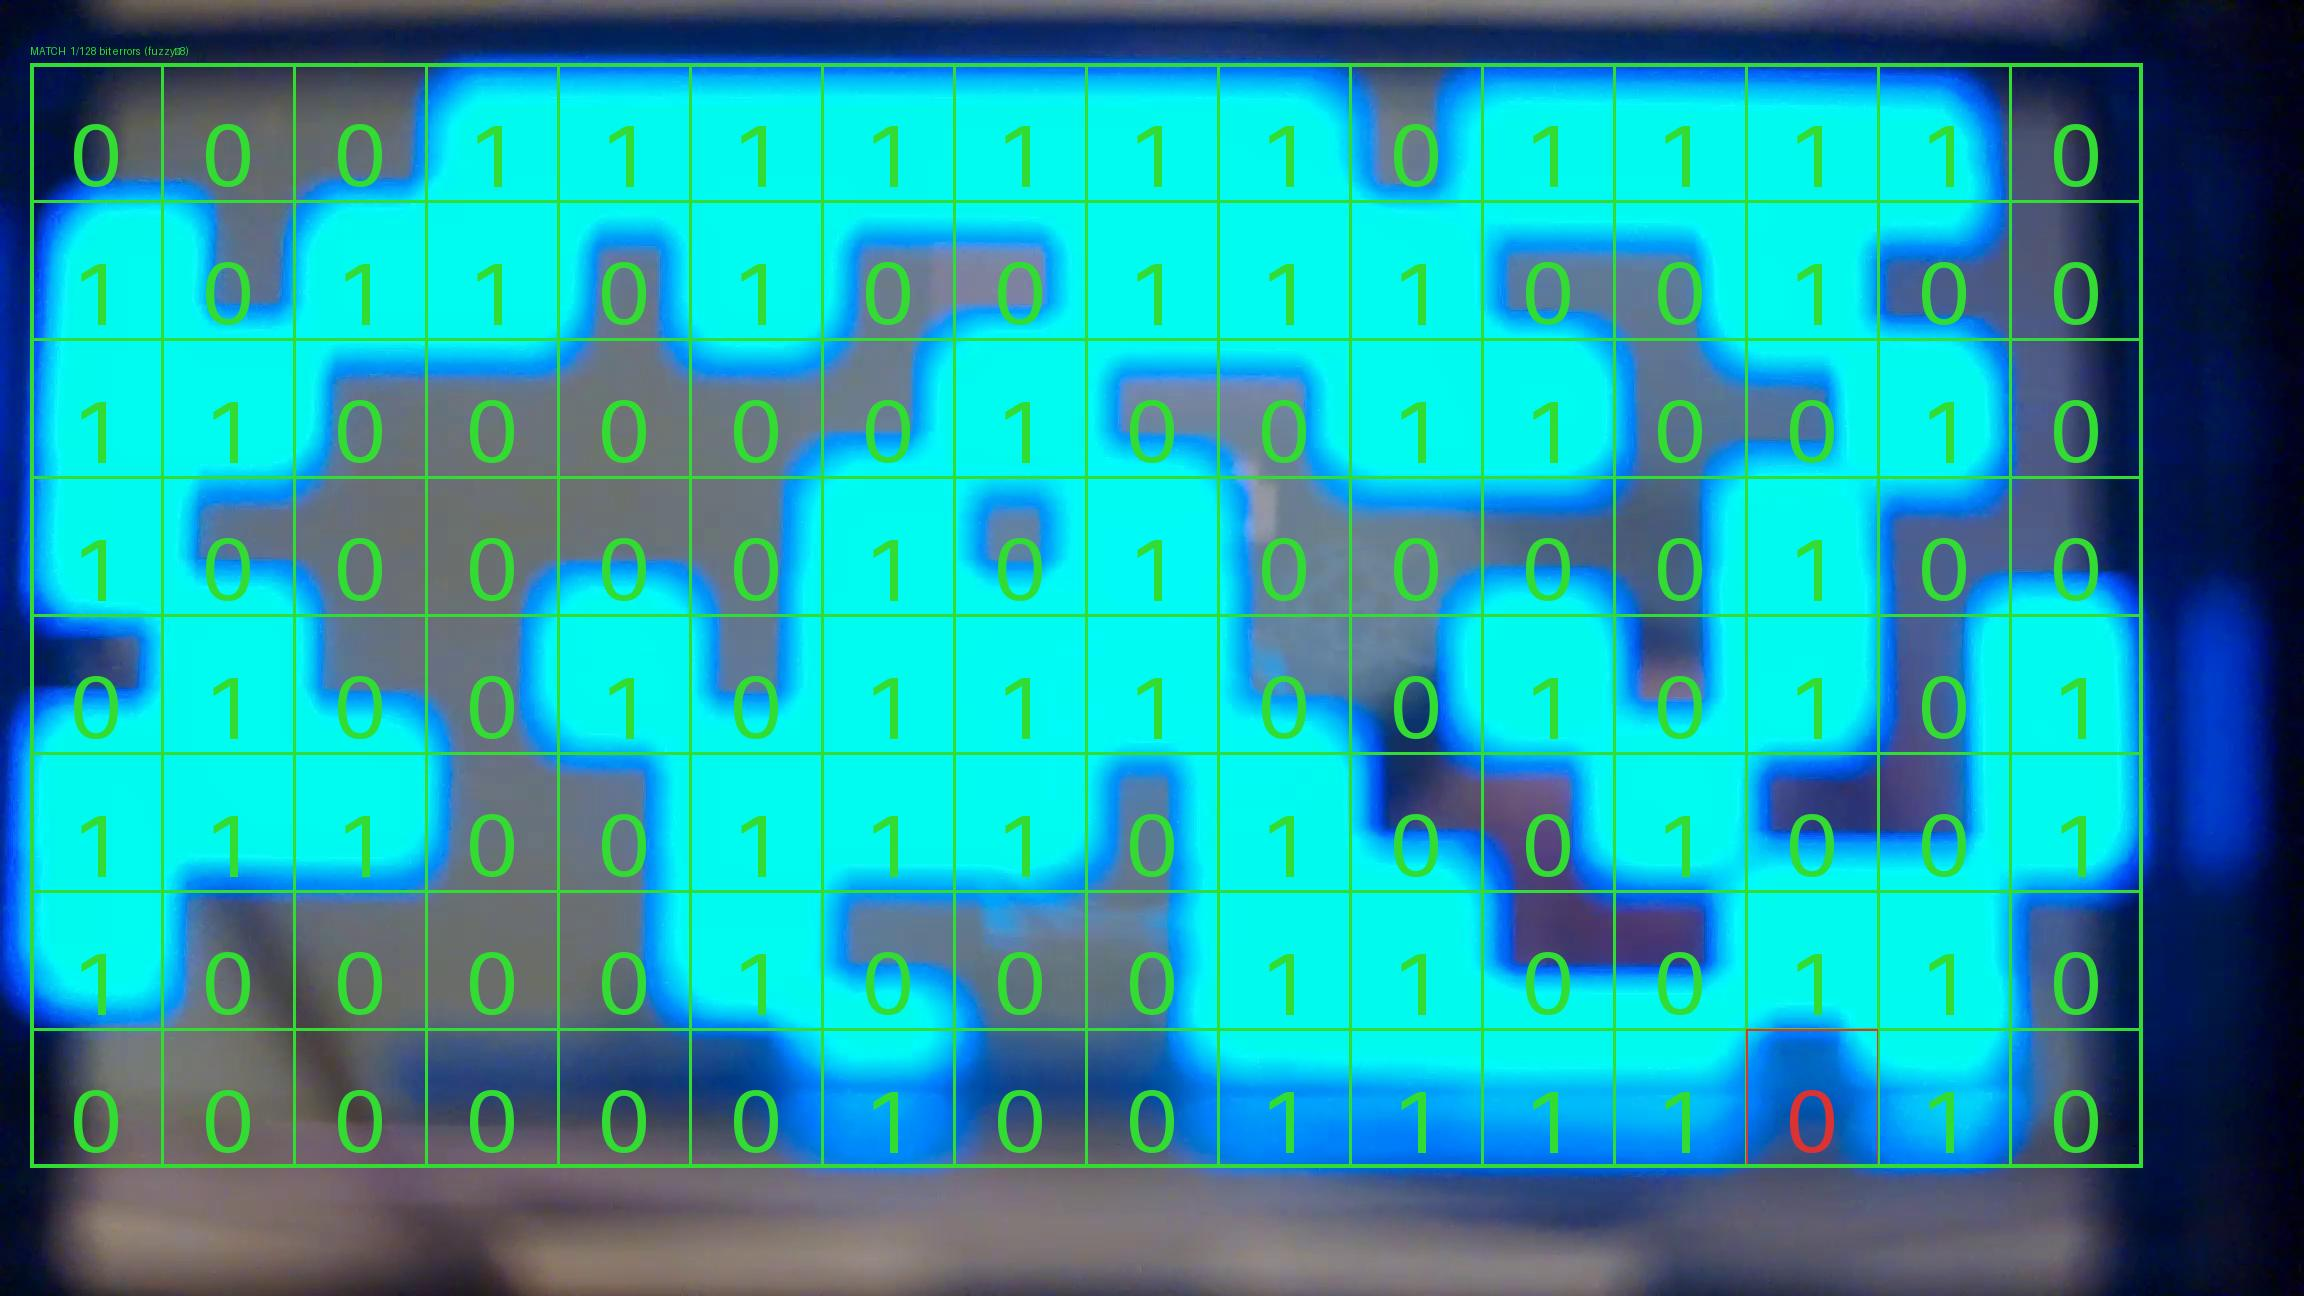
\includegraphics[width=0.49\linewidth]{frame_clean.jpg}%
  \hfill%
  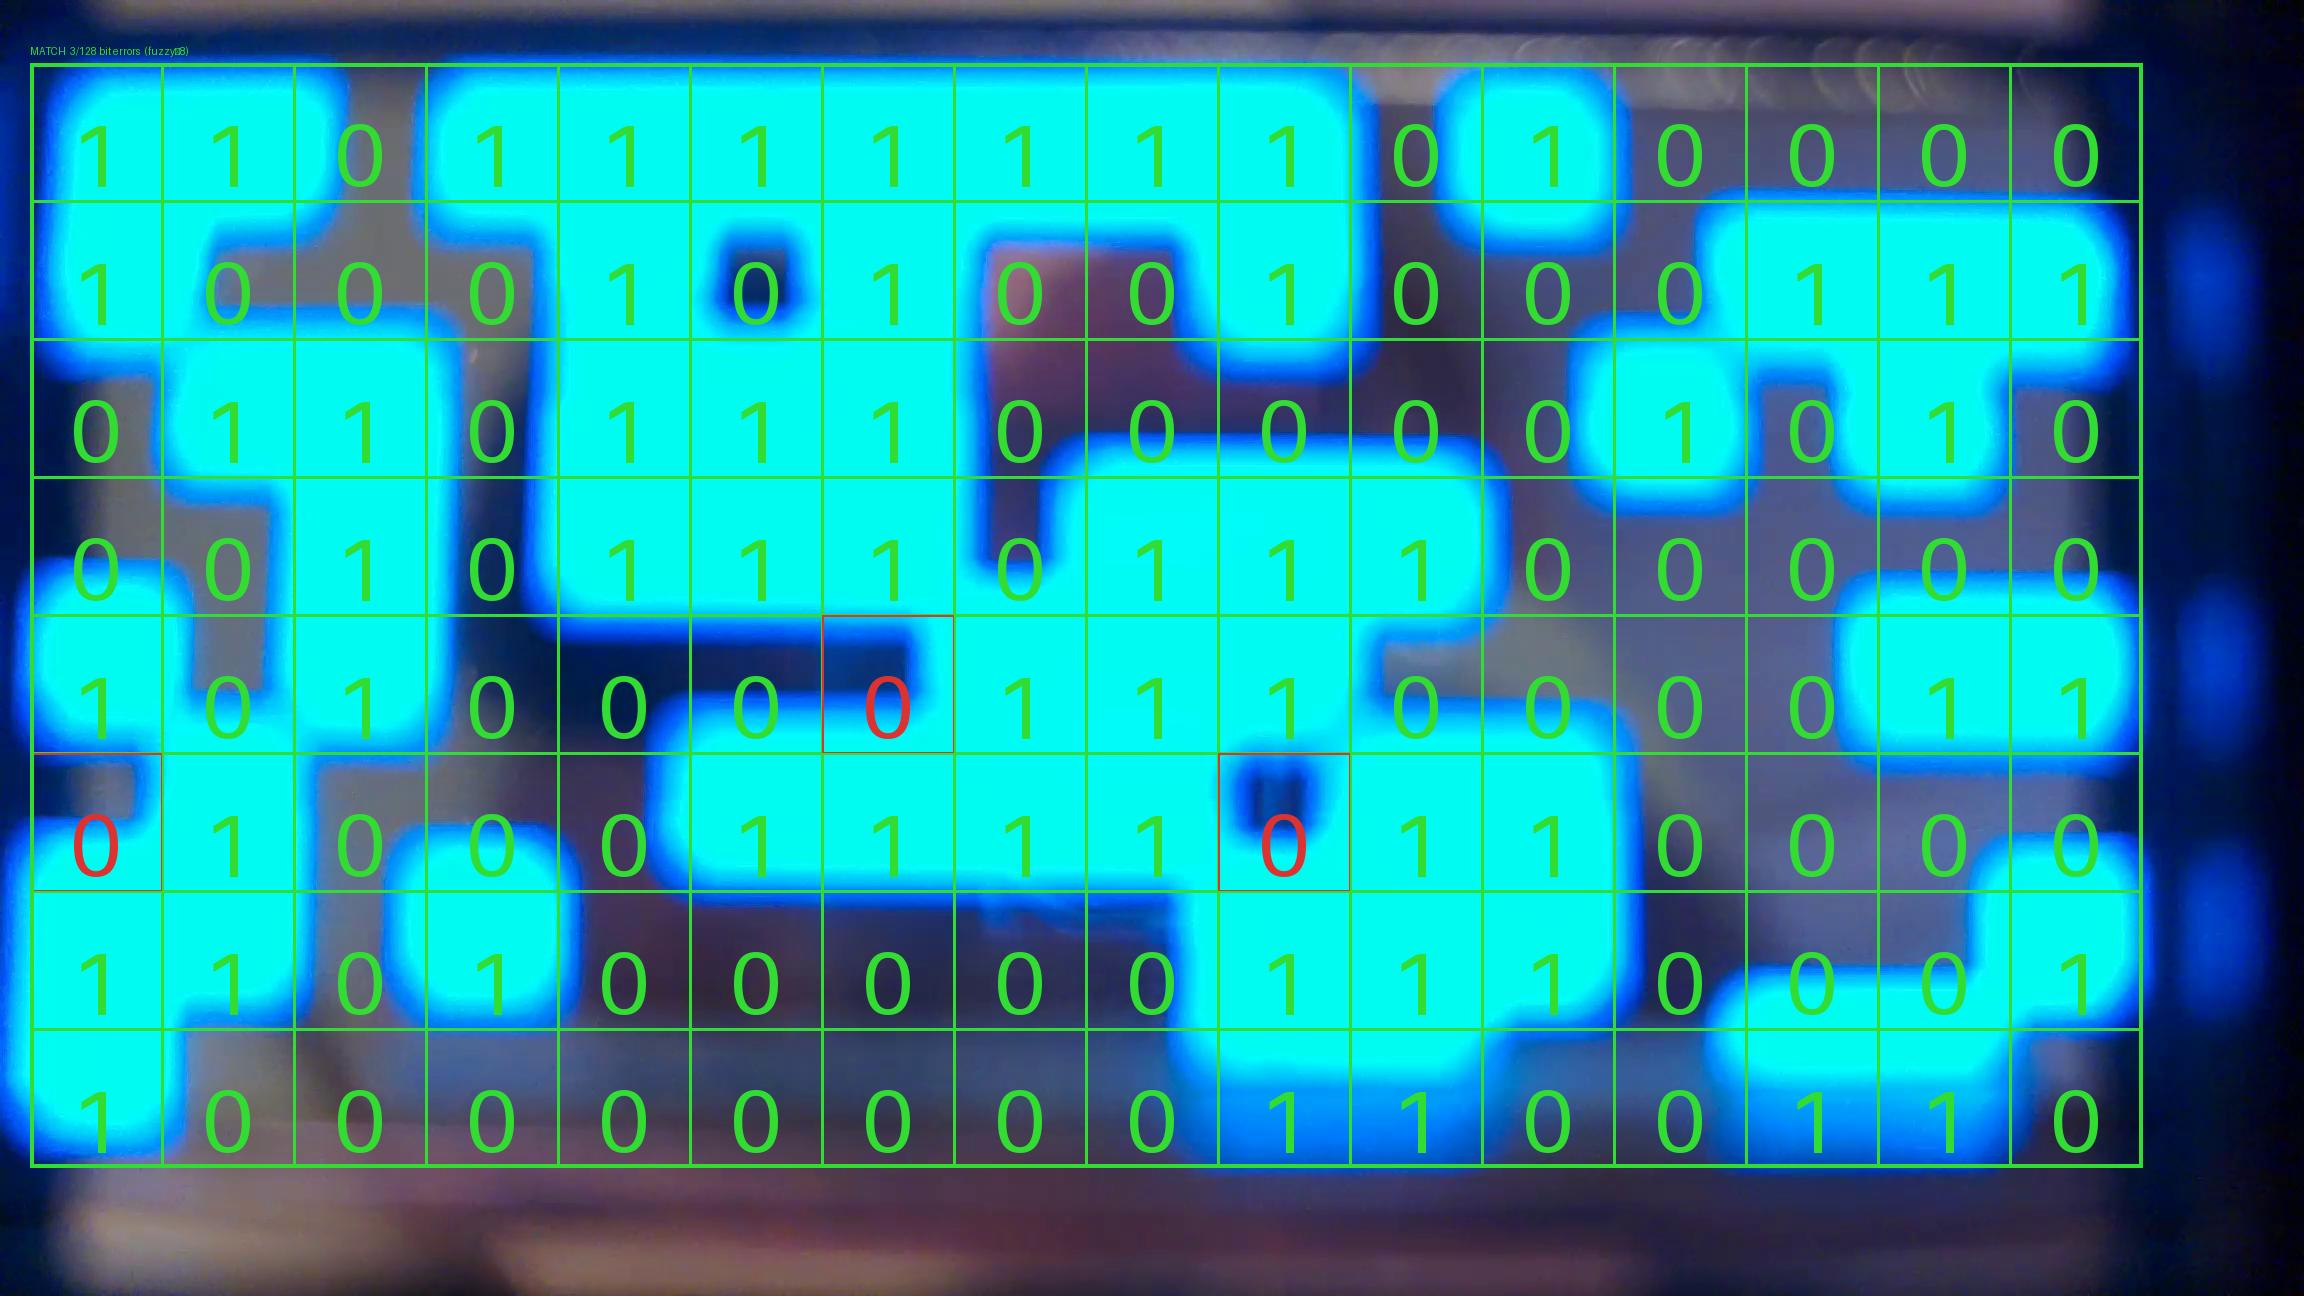
\includegraphics[width=0.49\linewidth]{frame_typical.jpg}
  \caption{Two blink cycles from the same recording. The 16$\times$8 grid is overlaid on the
    camera's view of the transparent OLED panel; green cells are correctly
    decoded bits, red cells are errors. The outer border is green when the
    decoded 128-bit value fuzzy-matches ($\leq$8 bit errors) the expected hash
    chain state, red otherwise. \textbf{Left:} best observed cycle (1/128 bit
    errors, 0.8\,\% BER). \textbf{Right:} typical cycle (3/128 bit errors,
    2.3\,\% BER). Both pass. Errors cluster at cell-boundary columns, consistent
    with a fixed sub-cell OLED-to-camera geometric offset rather than random
    optical noise.}
  \label{fig:debug}
\end{figure}



% ===========================================================================
\section{Security Analysis}
\label{sec:security}
% ===========================================================================

\textbf{Adversary capabilities.} We assume an adversary who can generate
photorealistic synthetic video and audio, splice or reorder frames, read public
ledger state at any time, and has full knowledge of the protocol. Computational
resources are unbounded for offline synthesis but bounded for real-time synthesis
(discussed in Section~\ref{sec:timebound}).

\textbf{Adversary goals.} The adversary wishes to produce content that falsely
claims to depict a real event, or that contains injected synthetic segments
(deepfaked face, cloned voice) within otherwise genuine content, with the edit
undetectable.

\textbf{Trust assumptions.} We assume ledger integrity (past blockhashes cannot be
rewritten; future ones cannot be predicted), sound cryptographic primitives
(SHA-256~\cite{nist-sha}), and that the capture device is not under adversarial
physical control during capture. We additionally assume the anchor broadcaster
supplies authentic blockhashes; a device should confirm~$H_0$ against a direct
Solana RPC query before beginning capture. PoR-Chain provides defense in depth
that supplements, rather than replaces, hardware roots of trust.

We analyze representative attack scenarios against PoR-Chain.

\subsection{Pure Deepfake Injection}

\textbf{Attack:} the adversary synthesizes content from scratch using a generative
model and submits it as if captured.

\textbf{Defense:} synthesized content does not contain any embedded signal.
Verification fails at step~3 of Algorithm~\ref{alg:verify} (decoded signal absent or
invalid).

\subsection{Frame Splicing}

\textbf{Attack:} the adversary takes genuine PoR-Chain content and removes,
reorders, or substitutes a subset of frames.

\textbf{Defense:} the cumulative hash chain breaks at the splice boundary.
Verification fails at step~4.

\subsection{Pre-Synthesis with Replay}

\textbf{Attack:} the adversary observes the ledger state at~$S_0$, synthesizes
content offline, then submits it claiming capture at $T_0 = \operatorname{time}(S_0)$.

\textbf{Defense:} unless the adversary can synthesize and submit a termination
anchor within $T_{\text{playback}} + W$ of~$T_0$, bidirectional time
bounding fails. Current diffusion-based video models require significantly more than real-time
compute per output-second on available hardware, making this attack infeasible
for content longer than a few seconds; however, this margin is expected to erode
as generative models improve.

\subsection{Lipsync Forgery}

\textbf{Attack:} the adversary takes genuine PoR-Chain video and overlays a
synthesized voice track.

\textbf{Defense (designed):} when dual-channel encoding is implemented, the audio
channel chain would mismatch the video channel chain (or fail verification
against~$H_0$ entirely). Acoustic encoding implementing this defense is planned
for future work.

\subsection{Voice Cloning Paired with Genuine Video}

\textbf{Attack:} adversary clones a target's voice, attaches it to a genuine
PoR-Chain video, and submits.

\textbf{Defense (designed):} when dual-channel encoding is implemented, the audio
chain check would fail identically to the lipsync forgery case.

\subsection{Optical Signal Replay Attack}

\textbf{Attack:} adversary records the OLED-emitted signal during a genuine capture,
then plays it back during a separate synthetic capture.

\textbf{Defense:} because $H_0$ is unique to each capture session and the chain is
deterministic from~$H_0$, replay of an old signal embeds an old chain. Bidirectional
time bounding (Section~\ref{sec:timebound}) detects the mismatch between the claimed
capture time and the actual ledger anchor time.

\subsection{Screen Relay Attack}

\textbf{Attack:} the adversary generates a synthetic scene using AI, plays it on a
screen, and places the screen in front of the PoR-Chain capture device. The camera
records the screen, which appears to be a real-world scene; the OLED hash signal is
overlaid and re-captured as normal. The resulting video passes all chain and time
bounding checks, because the physical feedback path requirement is genuinely
satisfied.

\textbf{Defense:} PoR-Chain does not currently detect this attack. The chain
verifies that the hash signal was physically re-captured, but cannot distinguish a
real three-dimensional scene from a flat screen displaying synthetic content.
Candidate mitigations include depth sensing (ToF, structured light, or stereo
vision) to confirm that the scene has physical three-dimensional extent, and
Moiré pattern detection to identify the pixel-grid interference artifacts that
appear when a camera photographs a digital display. Neither mitigation is
implemented in the reference build; both are directions for future work.

\subsection{Fuzzy-Matching Collision Probability}
\label{sec:fuzzy-prob}

The visual OLED check accepts a decoded 128-bit hash state if it falls within
Hamming distance~8 of any entry in the hash chain (\texttt{FUZZY\_BITS}~$= 8$).
This tolerance accommodates the systematic geometric decoding errors observed in
practice (1--6 bit errors per cycle; see Section~\ref{sec:impl}).
However, it raises the question of whether the threshold materially weakens
forgery resistance.

The probability that a uniformly random 128-bit string falls within Hamming
distance~8 of a fixed target is:
\[
  P_{\mathrm{fuzzy}}
  = \frac{\displaystyle\sum_{k=0}^{8}\binom{128}{k}}{2^{128}}
  = \frac{1{,}529{,}927{,}642{,}833}{2^{128}}
  \approx 4.5 \times 10^{-27}
  \approx 2^{-87.5}.
\]
This corresponds to an effective security level of 87.5~bits for the visual
check taken in isolation---a loss of roughly 40.5~bits relative to an exact
match, yet still far beyond any feasible brute-force budget.

\textbf{Multi-cycle compounding.}  The visual check does not verify a single
blink cycle: it verifies \emph{every} OLED-on cycle throughout the recording.
Each snapshot $H_n$ is a deterministic function of~$H_0$ and the preceding video
bytes, so fooling all cycles simultaneously requires finding a video whose
streaming SHA-256 snapshots all fall within 8~bits of the legitimate chain---a
problem equivalent to second-preimage resistance of SHA-256.
As intuition for the per-cycle difficulty under random guessing, the probability
that a uniformly random 128-bit string passes a single fuzzy check is
$P_{\mathrm{fuzzy}} \approx 4.5 \times 10^{-27} \approx 2^{-87.5}$; because the
chain states are not independently guessable, the joint probability across $N$
cycles is not simply $P_{\mathrm{fuzzy}}^N$ but is instead bounded by the
SHA-256 second-preimage hardness above.
The only computationally plausible approach is \emph{real-time synthesis}:
generating content while physically displaying the correct hash sequence on a
hardware OLED during capture, which is precisely the attack class the physical
feedback path is designed to make infeasible.

\textbf{Conjunctive check.}  The visual check is conjunctive with Check~1
(exact SHA-256 of the full compressed video stream), which provides 256-bit
preimage resistance independently.  An adversary must defeat both checks
simultaneously, so the combined security is bounded below by the stronger of
the two.

\subsection{Comparison with Prior Work}

\begin{table}[h]
\centering
\caption{Security property comparison}
\label{tab:comparison}
\begin{tabular}{lccccc}
\toprule
\textbf{Property} & \textbf{C2PA} & \textbf{PRNU} & \textbf{Watermarking}
  & \textbf{Timestamp} & \textbf{PoR-Chain} \\
\midrule
Resists post-hoc synthesis    & \textcolor{orange}{$\sim$} & \textcolor{orange}{$\sim$} & \textcolor{red}{$\times$}    & \textcolor{red}{$\times$} & \textcolor{green!60!black}{$\checkmark$} \\
Resists frame splicing        & \textcolor{orange}{$\sim$} & \textcolor{orange}{$\sim$} & \textcolor{orange}{$\sim$}  & \textcolor{red}{$\times$} & \textcolor{green!60!black}{$\checkmark$} \\
Resists lipsync forgery       & \textcolor{orange}{$\sim$} & \textcolor{red}{$\times$}  & \textcolor{orange}{$\sim$}  & \textcolor{red}{$\times$} & \textcolor{orange}{$\sim$} \\
Single-query verification     & \textcolor{green!60!black}{$\checkmark$} & n/a & \textcolor{green!60!black}{$\checkmark$} & \textcolor{green!60!black}{$\checkmark$} & \textcolor{green!60!black}{$\checkmark$} \\
Bidirectional time binding    & \textcolor{red}{$\times$} & \textcolor{red}{$\times$}  & \textcolor{red}{$\times$}   & \textcolor{red}{$\times$} & \textcolor{green!60!black}{$\checkmark$} \\
No hardware root of trust     & \textcolor{red}{$\times$} & \textcolor{green!60!black}{$\checkmark$} & \textcolor{orange}{$\sim$} & \textcolor{green!60!black}{$\checkmark$} & \textcolor{green!60!black}{$\checkmark^*$} \\
\bottomrule
\end{tabular}
\end{table}

\noindent$^*$PoR-Chain does not require a trusted signing key but does require a capture
device that supports physical signal emission and re-capture. $\sim$~denotes partial
or conditional resistance. For C2PA, $\sim$ indicates that post-hoc attacks are
detected (the content hash in the manifest breaks), but capture-time attacks---such
as recording a screen displaying synthetic content---are not.

% ===========================================================================
\section{Discussion and Future Work}
% ===========================================================================

\subsection{Standardization}

PoR-Chain is complementary to existing standards. The framework can be expressed as
a C2PA assertion type, with the initial anchor~$H_0$ and termination slot recorded in
the manifest. Adoption by C2PA, JPEG Trust, or a similar consortium would enable
interoperable verification.

\subsection{Privacy Considerations}

Content privacy is preserved by design: only the file hash of the captured content
and the anchor slot number~$S_0$ are recorded on-chain under the user's public key.
The file hash is a one-way digest that reveals nothing about the video content.
$H_0$ is already a publicly known Solana blockhash and discloses nothing beyond
what the ledger already publishes.

Two residual metadata exposures remain. First, recording $S_0$ on-chain reveals the
approximate capture time to within one Solana slot ($\approx$400\,ms); this is an
inherent consequence of the temporal-anchoring design and is acceptable in most
provenance use cases where capture time is intended to be verifiable. Second, the
submitting public key pseudonymously links multiple recordings to the same author;
users who require stronger unlinkability may submit termination anchors through a
privacy-preserving relay or use a fresh keypair per session.

\subsection{Limitations}
\label{sec:limitations}

\textbf{Hardware requirement.} The framework requires a capture device with both
signal emission and signal re-capture capabilities. Standalone software
implementations are not possible.

\textbf{Network dependency at beginning and end.} Network connectivity is required
only at the beginning of a recording---to fetch the initial anchor~$H_0$---and at
the end, to post the termination anchor. No connection is needed during capture.

\textbf{Partial optical encoding.} The current OLED codec encodes only the first
128 bits of the 256-bit hash state, constrained by the 128$\times$64-pixel
display. A higher-resolution display or an alternating two-frame scheme would
expose the full 256 bits.

\textbf{Controlled-environment assumption.} Decoding accuracy has been
characterized in a laboratory setting (fixed geometry, stable lighting). Field
robustness under varying illumination, camera motion, and platform re-encoding
is an open empirical question.

\textbf{Unimplemented components.} Acoustic encoding, dual-channel binding,
and verifier-side bidirectional time bounding are not yet built.

\subsection{Open Evaluation Directions}

We anticipate empirical evaluation along several axes, with results to be reported
in a follow-up paper:
\begin{itemize}
  \item Bit error rate of optical encoding under varying lighting conditions, and
    acoustic encoding when implemented.
  \item End-to-end verification latency on commodity hardware.
  \item Robustness against re-encoding by commercial video platforms.
  \item User study of perceptual impact of optical signal embedding.
\end{itemize}

% ===========================================================================
\section{Conclusion}
% ===========================================================================

We have presented PoR-Chain, a cryptographic framework for proving that multimedia
content was captured at a specific time and through a specific physical capture
process. The framework addresses a fundamental gap in existing provenance
schemes by binding content to a physical feedback path that no software-only
adversary can reproduce, and by anchoring the resulting hash chain to a public ledger
in a way that supports efficient verification and tamper-evident sequence integrity.
Bidirectional time bounding and dual-channel encoding are designed to extend the
framework to defeat increasingly sophisticated synthesis and forgery attacks;
acoustic encoding implementing the dual-channel design is planned for future work.

% ===========================================================================
\section*{Patent Disclosure}
% ===========================================================================

This work is the subject of the following Korean patent applications filed with the
Korean Intellectual Property Office (KIPO):

\begin{itemize}
  \item KR 10-2026-0083791 (Cumulative Hash Chain extension, filed 2026-05-08).
\end{itemize}

International filings under the Patent Cooperation Treaty are anticipated within the
priority window.

% ===========================================================================
% ===========================================================================
\bibliographystyle{plain}
\begin{thebibliography}{99}

\bibitem{por}
S.~Kim.
\newblock Proof of Reality: Binding Multimedia Content to Physical Capture
  through Ledger-Anchored Feedback Paths.
\newblock Preprint, KANT Labs, May 2026.
\newblock \url{https://doi.org/10.5281/zenodo.20205320}

\bibitem{c2pa}
Coalition for Content Provenance and Authenticity.
\newblock C2PA Technical Specification, v1.4, 2024.
\newblock \url{https://c2pa.org/specifications/}

\bibitem{prnu}
J.~Lukas, J.~Fridrich, and M.~Goljan.
\newblock Digital camera identification from sensor pattern noise.
\newblock \emph{IEEE Transactions on Information Forensics and Security},
  1(2):205--214, 2006.

\bibitem{lamport}
L.~Lamport.
\newblock Password authentication with insecure communication.
\newblock \emph{Communications of the ACM}, 24(11):770--772, 1981.

\bibitem{nist-sha}
National Institute of Standards and Technology.
\newblock Secure Hash Standard (SHS).
\newblock FIPS Publication 180-4, 2015.

\bibitem{solana}
A.~Yakovenko.
\newblock Solana: A new architecture for a high performance blockchain.
\newblock Whitepaper, 2018.
\newblock \url{https://solana.com/solana-whitepaper.pdf}

\end{thebibliography}

\end{document}
